\noindent

\includegraphics[height=1.25cm]{images/pictograms/benchmark}

\includegraphics[height=1.25cm]{images/pictograms/tools}

\includegraphics[height=1.25cm]{images/pictograms/FEM}

\includegraphics[height=1.25cm]{images/pictograms/paraview}

\includegraphics[height=1.25cm]{images/pictograms/clean}

%%%%%%%%%%%%%%%%%%%%%%%%%%%%%%%%%%%%%%%%%%%%%%%%%%%%%%%%%%%%%%%%%%%%%%%%%%%%%%%%%%%%%%%%%%%%%%%%%%%

\begin{flushright} {\tiny {\color{gray} python\_codes/fieldstone\_182/text.tex}} \end{flushright}

\par\noindent\rule{\textwidth}{0.4pt}

\begin{center}
\inpython
{\small Code: \url{https://github.com/cedrict/fieldstone/tree/master/python_codes/fieldstone_182}}
\end{center}

\par\noindent\rule{\textwidth}{0.4pt}

Last revision: March. 17th, 2026.

\par\noindent\rule{\textwidth}{0.4pt}

%%%%%%%%%%%%%%%%%%%%%%%%%%%%%%%%%%%%%%%%%%%%%%%%%%%%%%%%%%%%%%%%%%%%%%%%%%%%%%%%%%%%%%%%%%%%%%%%%%%

This \stone is the direction continuation of \stone 181. Please refer to it first.
This \stone compares three different ways of assembling the Stokes matrix
which are in essence identical to \stone 181.
The main difference between this \stone and \stone 181 lies in internal storage.

For example, the elemental matrices of stone 181 are defined as follows:
\begin{lstlisting}
K_el =np.zeros((ndof_V_el,ndof_V_el),dtype=np.float64)
G_el=np.zeros((ndof_V_el,m_P),dtype=np.float64)
f_el =np.zeros((ndof_V_el),dtype=np.float64)
h_el=np.zeros((m_P),dtype=np.float64)
\end{lstlisting}

while they are defined as follows in this stone:
\begin{lstlisting}
A_el=np.zeros((ndof_el,ndof_el),dtype=np.float64)
b_el=np.zeros(ndof_el,dtype=np.float64)
\end{lstlisting}

This translates for example in rather different loops in order to apply boundary conditions:
\begin{lstlisting}
for ikk in range(0,ndof_V_el):
    m1=local_to_global_V[ikk,iel]
    if bc_fix_V[m1]:
           K_ref=K_el[ikk,ikk] 
           for jkk in range(0,ndof_V_el):
               f_el[jkk]-=K_el[jkk,ikk]*bc_val_V[m1]
               K_el[ikk,jkk]=0
               K_el[jkk,ikk]=0
           K_el[ikk,ikk]=K_ref
           f_el[ikk]=K_ref*bc_val_V[m1]
           h_el[:]-=G_el[ikk,:]*bc_val_V[m1]
           G_el[ikk,:]=0
\end{lstlisting}
vs
\begin{lstlisting}
for i in range(0,ndof_V_el):
    idof=local_to_global[i,iel]
    if bc_fix_V[idof]:
       A_ref=A_el[i,i] 
       b_el[0:ndof_el]-=A_el[0:ndof_el,i]*bc_val_V[idof]
       b_el[i]=A_ref*bc_val_V[idof]
       A_el[i,:]=0
       A_el[:,i]=0
       A_el[i,i]=A_ref
\end{lstlisting}

Likewise the assembly process is much more concise in this stone than in the 
previous one. 

The question to be answered now is whether the reorganisation of the internal storage 
has any bearing on cpu times.

In what follows dashed lines are results obtained with \stone~181.


\begin{center}
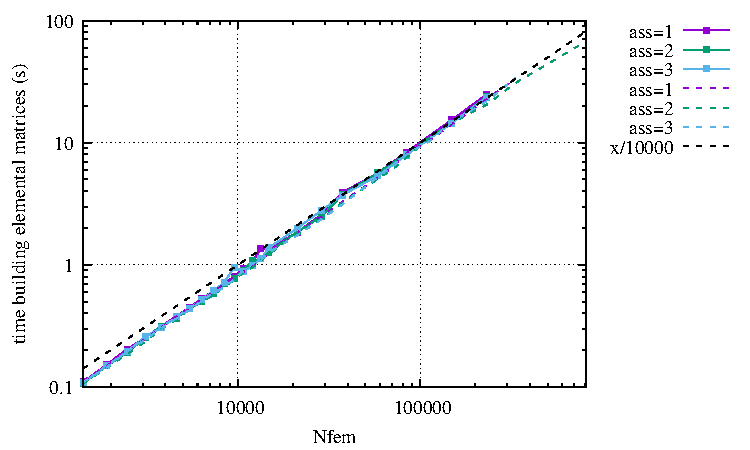
\includegraphics[width=10cm]{python_codes/fieldstone_182/RESULTS/times_matrices.pdf}
\end{center}

\begin{center}
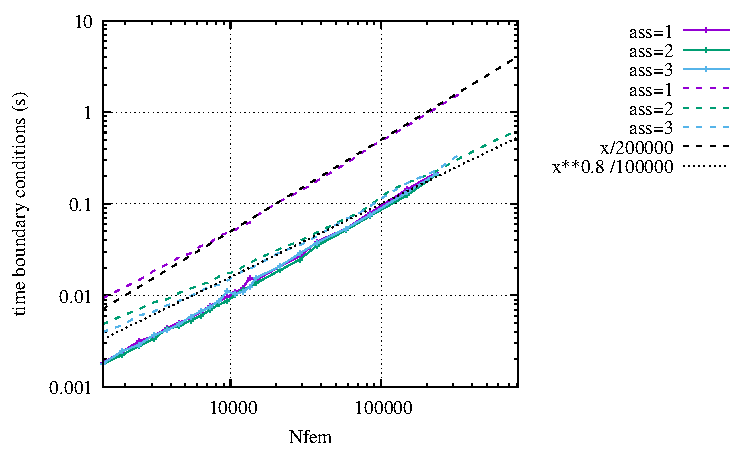
\includegraphics[width=10cm]{python_codes/fieldstone_182/RESULTS/times_bc.pdf}
\end{center}

\begin{center}
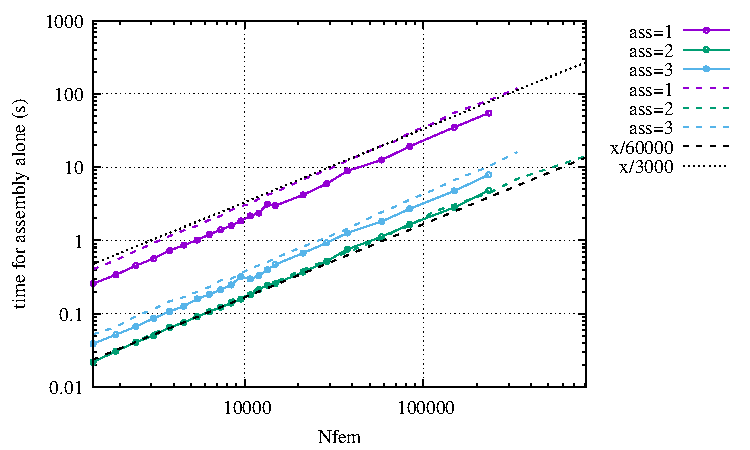
\includegraphics[width=10cm]{python_codes/fieldstone_182/RESULTS/times_assembly.pdf}
\end{center}

\begin{center}
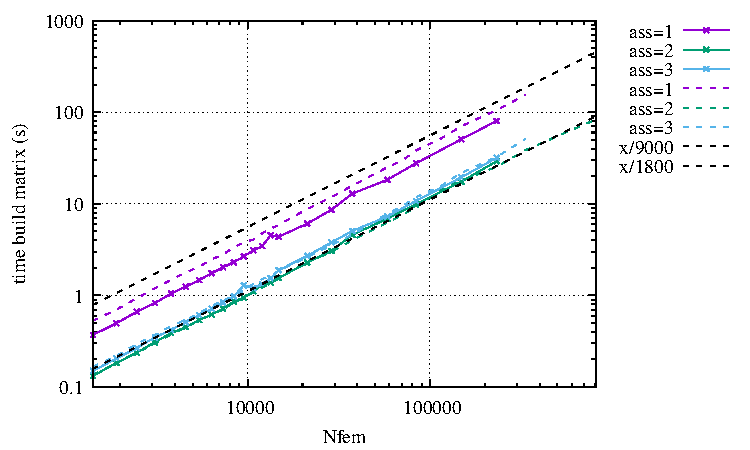
\includegraphics[width=10cm]{python_codes/fieldstone_182/RESULTS/times_build.pdf}
\end{center}

\begin{center}
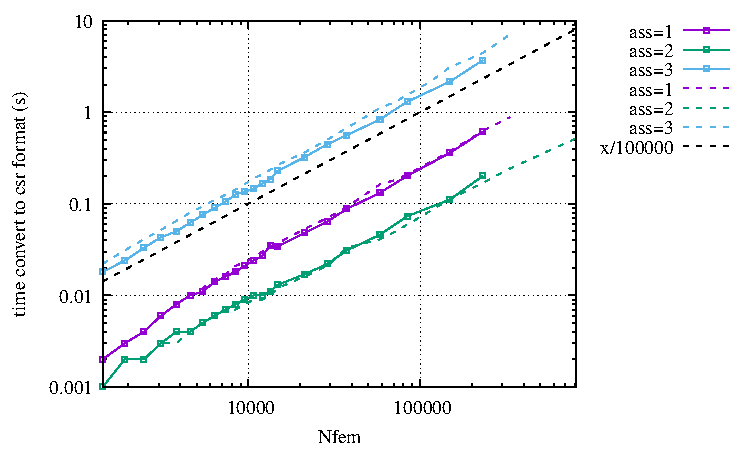
\includegraphics[width=10cm]{python_codes/fieldstone_182/RESULTS/times_convert.pdf}
\end{center}

\begin{center}
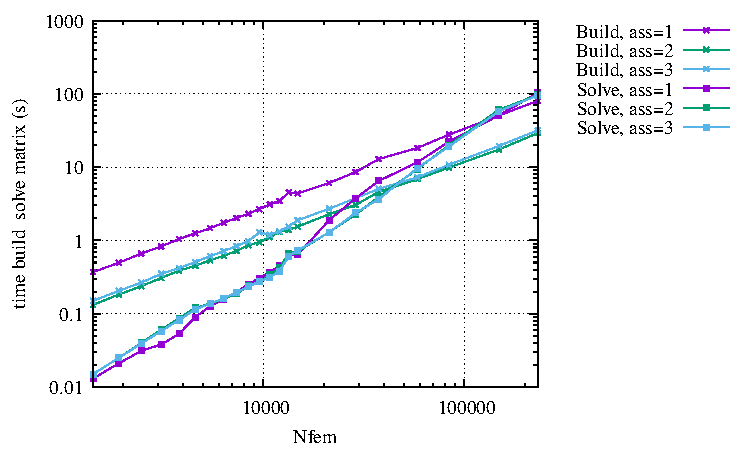
\includegraphics[width=10cm]{python_codes/fieldstone_182/RESULTS/times_build_solve.pdf}
\end{center}

\noindent 
\includegraphics[width=2.5cm]{./images/conclusion.png}

